\documentclass[10pt,twoside]{article}
\usepackage[utf8]{inputenc}
\usepackage{amsmath}
\usepackage{amsfonts}
\usepackage{amssymb}
\usepackage[spanish,es-noshorthands]{babel}
\usepackage[T1]{fontenc}
\usepackage{lmodern}
\usepackage{graphicx,hyperref}
\usepackage{tikz,pgf}
\usepackage{multicol}
\usepackage{subfig}
\usepackage[papersize={6.5in,8.5in},width=5.5in,height=7in]{geometry}
\usepackage{fancyhdr}
\pagestyle{fancy}
\fancyhead[LE]{
\includegraphics[height=12pt]{Images/logo-colegio.png} Matemáticas $11^{\circ}$}
\fancyhead[RE]{}
\fancyhead[RO]{\textit{Germ\'an Avenda\~no Ram\'irez, Lic. U.D., M.Sc. U.N.}}
\fancyhead[LO]{}

\author{Germ\'an Avenda\~no Ram\'irez, Lic. U.D., M.Sc. U.N.}
\title{\begin{minipage}{.2\textwidth}

\includegraphics[height=1.75cm]{Images/logo-colegio.png}\end{minipage}
\begin{minipage}{.55\textwidth}
\begin{center}
Taller de Nivelación 2014\\
Matemáticas $11^{\circ}$
\end{center}
\end{minipage}\hfill
\begin{minipage}{.2\textwidth}

\includegraphics[height=1.75cm]{Images/logo-sed.png} 
\end{minipage}}
\date{}
\begin{document}
\maketitle
Nombre: \hrulefill Curso: \underline{\hspace*{44pt}} Fecha: \underline{\hspace*{2.5cm}}
\let\ds\displaystyle
\section*{N\'{u}meros reales}
\begin{enumerate}
\item 
\begin{enumerate}
\item Grafique el intervalo $(-5,3)$ y $(2,\infty)$ en la recta real
\item Exprese las desigualdades $x\leq 3$ y $-1\leq x<4$ en notación de intervalos
\item Encuentre la distancia entre $-7$ y $9$ sobre la recta real
\end{enumerate}
\item Evalúe cada expresión
\begin{enumerate}
\begin{multicols}{5}
\item $(-3)^{4}$ \item $-3^{4}$ \item $\dfrac{5^{23}}{5^{24}}$ \item $\left(\dfrac{3}{3}\right)^{-2}$ \item $16^{-3/4}$
\end{multicols}
\end{enumerate}
\item Escriba cada n\'{u}mero en notaci\'{o}n cient\'{i}fica
\begin{enumerate}
\begin{multicols}{2}
\item 186\,000'000\,000 \item 0.0000003965
\end{multicols}
\end{enumerate}
\item Simplifique cada expresión. Escriba su respuesta final sin exponentes negativos
\begin{enumerate}
\begin{multicols}{3}
\item $\sqrt{200}-\sqrt{32}$ \item $(3a^{3}b^{3})(4ab^{2})^{2}$ \item $\left(\dfrac{3x^{3/2}y^{3}}{x^{2}y^{-1/2}}\right)^{-2}$
\item $\dfrac{x^{2}+3x+2}{x^{2}-x-2}$
\item $\dfrac{x^{2}}{x^{2}-4}-\dfrac{x+1}{x+2}$
\item $\dfrac{\frac{y}{x}-\frac{x}{y}}{\frac{1}{y}-\frac{1}{x}}$
\end{multicols}
\end{enumerate}
\item Racionalice el denominador y simplifique: $\dfrac{\sqrt{10}}{\sqrt{5}-2}$
\item Realice las operaciones indicadas y simplifique:
\begin{enumerate}
\begin{multicols}{3}
\item $3(x+6)+4(2x-5)$
\item $(x+3)(4x-5)$
\item $(\sqrt{a}+\sqrt{b})(\sqrt{a}-\sqrt{b})$
\item $(2x+3)^{2}$
\item $(x+2)^{3}$
\end{multicols}
\end{enumerate}
\item Factorice completamente cada expresión
\begin{enumerate}
\begin{multicols}{3}
\item $4x^{2}-25$
\item $2x^{2}+5x-12$
\item $x^{3}-3x^{2}-4x+12$
\item $x^{4}+27x$
\item $3x^{3/2}-9x^{1/2}+6x^{-1/2}$
\item $x^{3}y-4xy$
\end{multicols}
\end{enumerate}
\item Encuentre las soluciones reales:
\begin{enumerate}
\begin{multicols}{3}
\item $x+5=14-\frac{1}{2}x$
\item $\dfrac{2x}{x+1}=\dfrac{2x-1}{x}$
\item $x^{2}-x-12=0$
\item $2x^{2}+4x+1=0$
\item $\sqrt{3-\sqrt{x+5}}=2$
\item $x^{4}-3x^{2}+2=0$
\item $3|x-4|=10$
\end{multicols}
\end{enumerate}
\item Mary condujo de Bogotá a Melgar a una rapidez promedio de 80 km/h. De regreso, ella condujo en promedio a 70 km/h. El tiempo total de viaje fue de $4\frac{2}{3}$ de hora. Encuentre la distancia entre las dos ciudades.
\item Una lote rectangular tiene 70 m más de largo que de ancho y su diagonal mide 130 m. Encuentre las dimensiones del lote.
\item Solucione cada inecuación. Escriba la respuesta usando la notación de intervalos y dibuje la solución en la recta real.
\begin{enumerate}
\begin{multicols}{2}
\item $-4<5-3x\leq 17$
\item $x(x-1)(x+2)>0$
\item $|x-4|<3$
\item $\dfrac{2x-3}{x+1}\leq 1$
\end{multicols}
\end{enumerate}
\item Una botella de medicina debe ser guardada a una temperatura entre $5^{\circ}$C y 10$^{\circ}$C. Qué rango correspondería si se toma la escala Fahrenheit? (Recuerde que la temperatura en Fahrenheit (F) y Celsius (C) satisface la relación $C=\frac{5}{9}(F-32)$
\section*{Funciones}
\item Sea $f(x)=x^{2}-4x$ y $g(x)=\sqrt{x+4}$, encuentre:
\begin{enumerate}
\item El dominio de $f$ y el dominio de $g$
\item $f(-2)$, $f(0)$, $f(4)$, $g(0)$, $g(8)$, $g(-6)$
\item $f(x+2)$, $g(x+2)$, $f(2+h)$
\item La razón de cambio de $g$ entre $x=5$ y $x=21$. (Recuerde que la razón de cambio entre los extremos $x_{1}$ y $x_{2}$ se define como $\dfrac{f(x_{2})-f(x_{1}}{x_{2}-x_{1}}$
\item $f(g)$, $g(f)$, $f(g(12))$, $g(f(12))$
\end{enumerate}
\item Sea 
$
f(x)= \left\{ \begin{array}{lcl}
4 & \mbox{ si } & x\leq 2 \\
x-1 & \mbox{ si } & x>0
\end{array}
\right.
$
\begin{enumerate}
\item Evalúe $f(0)$, $f(1)$, $f(2)$, $f(3)$ y $f(4)$
\item Haga la gráfica de $f$
\end{enumerate}
\item Sea $f$ la función cuadrática $f(x)=-2x^{2}+8x+5$.
\begin{enumerate}
\item Exprese $f$ en la forma estandar (La forma estandard de la función $f(x)=ax^{2}+bx+c$, es $f(x)=a(x-h)+k$, que se obtiene completando el cuadrado donde el vértice está dado por el punto $(h,k)$)
\item Encuentre los valores máximo y mínimo de la función $f$
\item Haga la gráfica de $f$
\item Encuentre el intervalo en el cual $f$ es creciente y el intervalo en el cual $f$ es decreciente
\item ¿Cómo es la gráfica de la función $g(x)=-2x^{2}+8x+10$ respecto de la función $f$?
\item ¿Cómo es la gráfica de la función $h(x)=-2(x+3)^{2}+8(x+3)+5$ con respecto a la función $f$?
\end{enumerate}
\item Sin usar dispositivos electrónicos, encuentre la correspondencia entre las ecuaciones siguientes y las gráficas que se dan. Explique las razones de su elección.
\begin{itemize}
\begin{multicols}{3}
\item $f(x)=x^{3}-8x$
\item $g(x)=-x^{4}+8x^{2}$
\item $h(x)=x^{2}-5$
\item $k(x)=2^{-x}+3$
\item $r(x)=\dfrac{2x+3}{x^{2}-9}$
\item $s(x)=\dfrac{2x-3}{x^{2}+9}$
\end{multicols}
\end{itemize}
\begin{center}
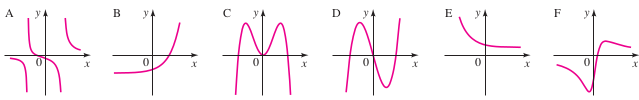
\includegraphics[scale=.6]{Images/funciones_2014-11-17_14:27:06.png} 
\end{center}
\item Una suma de \$25\,000 es depositada en una cuenta que paga 5.4\% de interés compuesto por año.
\begin{enumerate}
\item ¿Cu\'{a}nto ser\'{a} el monto en la cuenta despu\'{e}s de 3 años?
\item ¿Cu\'{a}ndo la cuenta tendr\'{a} un saldo que ascienda a \$35\,000?
\item ¿En cu\'{a}nto tiempo el dep\'{o}sito inicial se duplicar\'{a}?
\end{enumerate}
\section*{Sucesiones y progresiones}
Para las secuencias dadas en \ref{first}--\ref{second}
\begin{enumerate}
\item Encuentre los cinco primeros términos para la sucesión dada.
\item ¿Cuál es la diferencia común $d$?
\item Grafique los términos que encuentre en \textit{a)}
\end{enumerate}
\begin{multicols}{2}
\item $a_{n}=5+2(n-1)$\label{first}
\item $a_{n}=3-4(n-1)$
\item $a_{n}=\frac{5}{2}-(n-1)$
\item $a_{n}=\frac{1}{2}(n-1)$\label{second}
\end{multicols}
\ref{third}--\ref{fourth} Encuentre el $n-\'{e}simo$ t\'{e}rmino de la progresi\'{o}n aritm\'{e}tica dado el primer t\'{e}rmino $a_{1}$ y la diferencia com\'{u}n $d$. ¿Cu\'{a}l es el d\'{e}cimo t\'{e}rmino?
 \begin{multicols}{2}
 \item $a_{1}=3$, $d=5$ \label{third} 
 \item $a_{1}=-6$, $d=3$
 \item $a_{1}=\frac{5}{2}$, $d=-\frac{1}{2}$
 \item $a_{1}=\sqrt{3}$, $d=\sqrt{3}$ \label{fourth}
 \end{multicols}
\item Determine la diferencia común, el quinto término, el n-ésimo término y el centésimo término de las progresiones aritméticas
\begin{enumerate}
\begin{multicols}{2}
\item 1, 5, 9, 13, \ldots
\item 11, 8, 5, 2, \ldots
\item $\frac{7}{6}$, $\frac{5}{3}$, $\frac{13}{6}$, $\frac{8}{3}$, \ldots
\item 15, 12.3, 9.6, 6.9, \ldots
\end{multicols}
\end{enumerate}
\item El décimo término de una progresión aritmética es $\frac{55}{2}$, y, el segundo término es $\frac{7}{2}$. Encuentre el primer término.
\item El duodécimo término de una progresión aritmética es 32, y el quinto término es 18. Encuentre el vigésimo término.

\begin{minipage}{.45\textwidth}
\item Los postes de teléfono son puestos en pila, con 25 postes en el primer nivel, 24 en el segundo y así sucesivamente. Si hay 12 niveles, ¿cuántos postes de teléfono contiene la pila de postes?
\end{minipage}\hfill
\begin{minipage}{.45\textwidth}
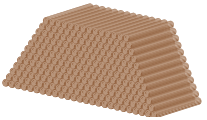
\includegraphics[scale=.9]{Images/postes.png} 
\end{minipage}
\ref{five}--\ref{eight} Dado el n-ésimo término de la progresi\'{o}n.
\begin{enumerate}
\item Encuentre los cinco primeros t\'{e}rminos
\item ¿Cu\'{a}l es la raz\'{o}n com\'{u}n $r$?
\item Grafique los t\'{e}rminos que encuentre en \textit{a)}
\end{enumerate}
\begin{multicols}{2}
\item $a_{n}=5(2)^{n-1}$\label{five}
\item $a_{n}=3(-4)^{n-1}$
\item $a_{n}=\frac{5}{2}\left(-\frac{1}{2}\right)^{n-1}$
\item $a_{n}=3^{n-1}$\label{eight}
\end{multicols}
\ref{nineth}--\ref{tenth} Determine si la sucesión es progresión geométrica. Si es, encuentre la razón común $r$
 \begin{multicols}{2}
\item 2, 6, 18, 36, \ldots \label{nineth}
\item 27, -9, 3, -1, \ldots
\item $e^{2}$, $e^{4}$, $e^{6}$, $e^{8}$, \ldots
\item $\frac{1}{2}$, $\frac{1}{4}$, $\frac{1}{6}$, $\frac{1}{8}$, \ldots \label{tenth}
 \end{multicols}
\item Las frecuencias de las notas musicales (medidas en ciclos por segundo) forman una progresión geométrica. El DO central tiene una frecuencia de 256, y el DO una octava arriba tiene una frecuencia de 512. Encuentre la frecuencia del DO dos octavas abajo del DO central.
\item Un cultivo de bacterias tiene inicialmente 5000 bacterias y su número aumenta 8\% cada hora. ¿Cuántas bacterias hay al cabo de 5 horas? Encuentre una expresi\'{o}n que indique el n\'{u}mero de bacterias que hay al cabo de $n$ horas.
\item Sea la función $f(x)=\left\{\begin{array}{lcl}
3 & \mbox{ si } & x<0\\
2 & \mbox{ si } & x=0\\
3-x \mbox{ si } & 0<x<2\\
x \mbox{ si } & x\geq 2
\end{array}\right.$
\begin{enumerate}
\section*{L\'{i}mites}
\item Grafique la funci\'{o}n $f$
\item Eval\'{u}e
\begin{enumerate}
\begin{multicols}{5}
\item $f(0)$
\item $\ds{\lim_{x\rightarrow 0}f(x)}$
\item $\ds{\lim_{x\rightarrow 1}f(x)}$
\item $\ds{\lim_{x\rightarrow 2^{-}}f(x)}$
\item $\ds{\lim_{x\rightarrow 2^{+}}f(x)}$
\end{multicols}
\end{enumerate}
\end{enumerate}
\item Evalúe los límites, si existen.
\begin{enumerate}
\begin{multicols}{3}
\item $\ds{\lim_{x\rightarrow 3}\dfrac{x^{2}+4x-21}{x-3}}$
\item $\ds{\lim_{x\rightarrow -3}\dfrac{x^{2}+4x-21}{x-3}}$
\item $\ds{\lim_{x\rightarrow 2}\dfrac{x^{2}+4}{x-2}}$
\end{multicols}
\end{enumerate}
\section*{Probabilidad}
\item La administración Federal de Ferrocarriles proporcionó las cinco categorías principales de violaciones para el ferrocarril CSX para los años 1999-2003 en la tabla siguiente. Hubo un total de 1897 violaciones. La información estuvo contenida en el artículo \textit{Democrat and Chronicle}, 29 de diciembre, 2004, titulado "Rail cop lacks a big stick". (El uniformado no lleva "garrote").
\begin{minipage}{.55\textwidth}
\begin{center}
\begin{tabular}{lc}
Categor\'{i}a & N\'{u}mero \\ 
\hline 
Seguridad en v\'{i}as & 485 \\ 
Equipo de seguridad en trenes & 324 \\ 
Horas de trabajo de empleados & 323 \\ 
Seguridad en furgones & 289 \\ 
Locomotoras & 248 \\ 
Todos los otros & 228 \\ 
\hline 
Total & 1897 \\ 
\end{tabular} 
\end{center}
\end{minipage}\hfill
\begin{minipage}{.4\textwidth}
Si una violación (infracción) se selecciona al azar para repaso, ¿cuál es la probabilidad de que la violación para el CSX se deba a lo siguiente?
\begin{enumerate}
\item Equipo de seguridad en trenes
\item Horas de trabajo de empleados
\item Seguridad en furgones o seguridad en vía.\\
 ¿Qué pasa si se seleccionan dos violaciones?
 \item ¿Sería esto un ejemplo de muestreo con o sin restitución? Explique por qué.
\end{enumerate}\end{minipage}

\item Mil personas seleccionadas de cierta enfermedad reciben un examen clínico. Como consecuencia del examen, la muestra de 1000 personas se clasifica de acuerdo con su estatura y situaci\'{o}n de su enfermedad.
\begin{center}
\begin{tabular}{lccccc}
 & \multicolumn{5}{c}{Situación de enfermedad} \\ \hline 
Estatura & Ninguno & Benigno & Moderado & Grave & Total \\ \hline
Alta & 122 & 78 & 139 & 61 & 400 \\ 
Media & 74 & 51 & 90 & 35 & 250 \\ 
Corta & 104 & 71 & 121 & 54 & 350 \\ 
\hline 
Total & 300 & 200 & 350 & 150 & 1000 \\ 
\hline 
\end{tabular} 

\end{center}Use la información de la tabla para estimar la probabilidad de ser de estatura media o corta y tener situación de enfermedad moderada o grave.
\end{enumerate}
\end{document}
